\section{Auswertung}
\label{sec:Auswertung}

Zunächst wird die in der Durchführung (\ref{sec:d0}) beschriebene Justierung durchgeführt.
Nach Bestimmung der Resonanzfrequenz des fest justieren Stromkreises sowie der Justierung des regelbaren Stromkreises ergibt sich eine Resonanzfrequenz von
\begin{align*}
\nu_{\text{res}} = \SI{30.49}{\kilo\hertz}.
\end{align*}
Der Theoriewert der Resonanzfrequenz berechnet sich nach \eqref{eqn:omega1} zu
\begin{align*}
  \nu_{\text{res,t}} = \SI{31.26}{\kilo\hertz},
\end{align*}
so dass sich eine relative Abweichung von $\nu_{\text{res}}$ zu $\nu_{\text{res,t}}$ von
\begin{align*}
  f_{\text{res}} = \SI{2.46}{\percent}
\end{align*}
ergibt.
Dabei wird die relative Abweichung eines Messwertes zu seinem Theoriewert hier und in allen folgenden Rechnungen nach
\begin{equation}
f = \frac{\lvert N - x \rvert }{N}
\label{eqn:rel_err}
\end{equation}
mit einem Theoriewert $N$ sowie einem Messwert $x$ berechnet.
\subsection{Bestimmung der Schwebungsfrequenzen}
Das Verhältnis der Resonanzfrequenzen $\omega_r$ und der Schwebungsfrequenzen $\omega_s$ wird, wie in der Durchführung (\ref{sec:d1}) beschrieben sowie in Abbildung \ref{fig:4} skizziert, bestimmt.

Tabelle \ref{tab:1} gibt die Messdaten sowie Theoriewerte an.

%\OverfullCenter{
\begin{table}
  \centering
  \caption{Messdaten für die Messung der Schwebungsfrequenzen}
  \label{tab:1}
  \sisetup{table-format=3.4}
  \begin{tabular}{c c c c c c c c c}
    \toprule
    {$N$} & {$ C_k [\si{\nano\farad}] $} & {$\increment C_k [\si{\nano\farad}] $} & {$ \omega_r [\si{\kilo\hertz}] $} & {$ \omega_s [\si{\kilo\hertz}] $} & {$\frac{\omega_r}{\omega_s}_{\text{}}$} & {$\increment \frac{\omega_r}{\omega_s}_{\text{}}$} & {f [\%]} \\
    \midrule
    \input{build/wr_ws_verhaeltnis.tex}
    \bottomrule
  \end{tabular}
\end{table}
%}


Hierbei beschreibt $N$ die Anzahl der Maxima der Resonanzfrequenz pro halber Periode der Schwebungsfrequenz, $C_K$ beschreibt die jeweils betrachtete Justierung des Koppelkondensators $C_k$.
Die Werte für $\omega_r$ und $\omega_s$ berechnen sich nach \eqref{eqn:omega_s} und \eqref{eqn:omega_r}, $\frac{\omega_r}{\omega_s}$ gibt das Verhältnis der beiden theoretischen Größen an.
Zuletzt wird die relative Abweichung der experimentell abgelesenen Werte zu den Theoriewerten angegeben.\\
Die hier berechneten Fehler sowie alle folgenden fehlerbehafteten Messgrößen berechnen sich nach dem Gaußschen Fehlerfortpflanzungsgesetz.
Für den Fehler von $\omega_r$ von $\omega_s$ ergibt sich die Fehlerformel
\begin{equation}
\increment{\omega_{r/s} = \frac{1}{ C_k^2 L \sqrt{ \frac{1}{C} + \frac{2}{C_k }  }   \increment{C_k}}}.
%  \increment{\omega_r} = \sqrt{ \Biggl( \frac{1}{2} \biggl( \frac{-C}{2 \sqrt{LC}^3 } - \frac{\frac{1}{C} + \frac{2}{C_k} }{2 L^2 \sqrt{ \frac{\frac{1}{C} + \frac{2}{C_k }}{L} } } \biggr)   \increment{L} \Biggr)^2 + \Biggl( \frac{1}{2} \biggl( \frac{-L}{2 \sqrt{LC}^3 } - \frac{1}{2 C^2 L \sqrt{ \frac{\frac{1}{C} + \frac{2}{C_k }}{L} } } \biggr)   \increment{C} \Biggr)^2  + \Biggl(\frac{-1}{ C_k^2 L \sqrt{ \frac{\frac{1}{C} + \frac{2}{C_k }}{L} } } \biggr)   \increment{C_k} \Biggr)^2   }
\end{equation}
Bei dem direkten Vergleich der Theoriewerte mit den abgelesenen Werten fällt eine systematische Abweichung auf, so dass $N$, abgesehen von den beiden Kondensatoren mit den größten Kapazitäten, eine Abweichung nach unten besitzt.
Um diesen Fehler zu beheben, wird nun bei der Berechnung der Theoriewerte ebenfalls die reale Kapazität $C_{\text{sp}}$ der Spule berücksichtigt.
Im Gegensatz zu \eqref{eqn:omega1} und \eqref{eqn:omega2} ergeben sich nun für die korrigierte Bestimmung
\begin{equation}
  \omega_{1'} = \frac{1}{\sqrt{L(C+C_{\text{sp}})}}
  \label{eqn:omega1_neu}
\end{equation}
sowie
\begin{equation}
  \omega_{2'} = \frac{ 1}{  \sqrt{\Bigl( \bigl( \frac{1}{C} + \frac{2}{C_k}  \bigr)^{-1} + C_{\text{sp}} \Bigr) L }}.
  \label{eqn:omega2_neu}
\end{equation}
Hiermit ergeben sich die in Tabelle \ref{tab:2} angegebenen Werte.
\begin{table}
  \centering
  \caption{Messdaten für die Messung der Schwebungsfrequenzen unter Berücksichtigung von $C_{\text{sp}}$}
  \label{tab:2}
  \sisetup{table-format=3.4}
  \begin{tabular}{c c c c c c c c c}
    \toprule
    {$N'$} & {$ C_k' [\si{\nano\farad}] $} & {$\increment C_k' [\si{\nano\farad}] $} & {$ \omega_r' [\si{\kilo\hertz}] $} & {$ \omega_s' [\si{\kilo\hertz}] $} & {$\frac{\omega_r'}{\omega_s'}_{\text{}}$} & {$\increment \frac{\omega_r'}{\omega_s'}_{\text{}}$} & {f' [\%]} \\
    \midrule
    \input{build/wr_ws_verhaeltnis_neu.tex}
    \bottomrule
  \end{tabular}
\end{table}

\subsection{Bestimmung der Fundamentalfrequenzen}

Die Fundamentalfrequenzen werden, wie in der Durchführung (\ref{sec:d2}) beschrieben mithilfe von Lissajous-Figuren bestimmt.
Der gemessene Wert von $\nu_{1,\text{gem}}$ wird für alle Koppelkondensatoren zu
\begin{align*}
  \nu_{1,\text{gem}} = \SI{30.30}{\kilo\hertz}
\end{align*}
bestimmt. Nach Formel \ref{eqn:omega1_neu} ergibt sich ein Theoriewert von
\begin{align*}
   \nu_{1,\text{ber}} = \SI{30.56}{\kilo\hertz},
\end{align*}
so dass sich eine relative Abweichung des experimentell bestimmten Wertes von $\nu_1$ zum Theoriewert von
\begin{align*}
  f_{\nu_1} = \SI{0.84}{\percent}
\end{align*}
ergibt.\\
Die Werte der zweiten Fundamentalfrequenz $\nu_2$ sind nach Formel \ref{eqn:omega2_neu} von der Kapazität des Koppelkondensators abhängig.
Dementsprechend werden in Tabelle \ref{tab:3} die gemessenen Fundamentalfrequenzen $\nu_{2,\text{gem}}$ sowie die mit Hilfe von \eqref{eqn:omega2_neu} bestimmten Werte $\nu_{2,\text{ber}}$ angegeben.
Zusätzlich wird die relative Abweichung der gemessenen zu den berechneten Frequenzwerten nach \eqref{eqn:rel_err} berechnet und angegeben.
\begin{table}[H]
  \centering
  \caption{Gemessene und berechnete Frequenzen}
  \label{tab:3}
  \sisetup{table-format=2.2}
  \begin{tabular}{c c c c c}
    \toprule
    {$C_k [\si{\nano\farad}]$} & {$\nu_{2,\text{gem}} [\si{\kilo\hertz}]$} & {$\nu_{2,\text{ber}} [\si{\kilo\hertz}]$} & {$\increment \nu_{2,\text{ber}} [\si{\kilo\hertz}]$} & {$f [\%]$} \\
    \midrule
    \input{build/vergleichdirekt.tex}
    \bottomrule
  \end{tabular}
\end{table}
Der Fehler von $\nu_{2,\text{ber}}$ berechnet sich zu
\begin{equation}
\increment{\nu_{2,\text{ber}}} =  \frac{C^2 L}{2\pi (2C+C_k)^2 \Bigl( \frac{L(C C_k + 2 C C_s + C_k C_s)}{2C+C_k} \Bigr)^{1.5} } \increment{C_k}.
\end{equation}
Für die gemessenen Frequenzen wird jeweils eine Messungenauigkeit von
\begin{align*}
  \increment \nu_{\text{gem}} = \SI{0,5}{\kilo\hertz}
\end{align*}
angenommen, da das digitale Oszilloskop nur diskrete Werte angibt.


\subsection{Bestimmung eines Frequenzspektrums}
Das Frequenzspektrum wird, wie in der Durchführung (\ref{sec:d3}) beschrieben, aufgenommen.
Der Koppelkondensator wird bei der durchgeführten Messung auf $C_k = \SI{1.01}{\nano\farad}$ eingestellt.
Der Frequenzgenerator erzeugt dabei eine Sinusspannung der Amplitude $U_0 = \SI{30}{\volt}$.
Innerhalb von einer Sekunde durchläuft der Frequenzgenerator den Bereich von $\nu_{\text{start}}$ bis $\nu_{\text{end}}$ mit
\begin{align*}
  \nu_{\text{start}} &= \SI{14.75}{\hertz} \\
  \nu_{\text{end}} &= \SI{84.39}{\kilo\hertz}.
\end{align*}
Die Peaks treten für
\begin{align*}
  \tau_1 &= \SI{360}{\milli\second} \\
  \tau_2 &= \SI{552}{\milli\second}.
\end{align*}
auf, wobei $\tau_1$ die Zeit vom Beginn des Frequenzdurchlaufes zum ersten Peak ist sowie $\tau_2$ die Zeit bis zum zweiten Peak.
Die Frequenzen der Peaks bestimmen sich für einen linearen Frequenzdurchlauf innerhalb von einer Sekunde durch
\begin{align}
  \nu_{\text{peak}} = (\nu_{\text{end}} - \nu_{\text{start}}) \tau + \nu_{\text{start}}.
\end{align}
Hieraus lassen sich die Frequenzen der Peaks bestimmen zu
\begin{align*}
  \nu_1 &= \SI{30390}{\hertz} \\
  \nu_2 &= \SI{46590}{\hertz}.
\end{align*}
Die relativen Abweichungen zu den nach \eqref{eqn:omega1_neu} bzw. \eqref{eqn:omega2_neu} bestimmten Theoriewerten ergeben sich nach \eqref{eqn:rel_err} zu
\begin{align*}
  f_{\nu_1} &= \SI{0.56}{\percent} \\
  f_{\nu_2} &= \SI{1.95}{\percent}.
\end{align*}
%Berechnet man zusätzlich die zu diesen Frequenzen erreichten Stromwerte, so erhalten wir nach \eqref{eqn:idoof}
%\begin{align*}
%  I_{2,1} &= \SI{0.0155}{\ampere} \\
%  I_{2,2} &= \SI{0.0103}{\ampere}.
%\end{align*}
%
%
%
%
%\begin{figure}
%  \centering
%  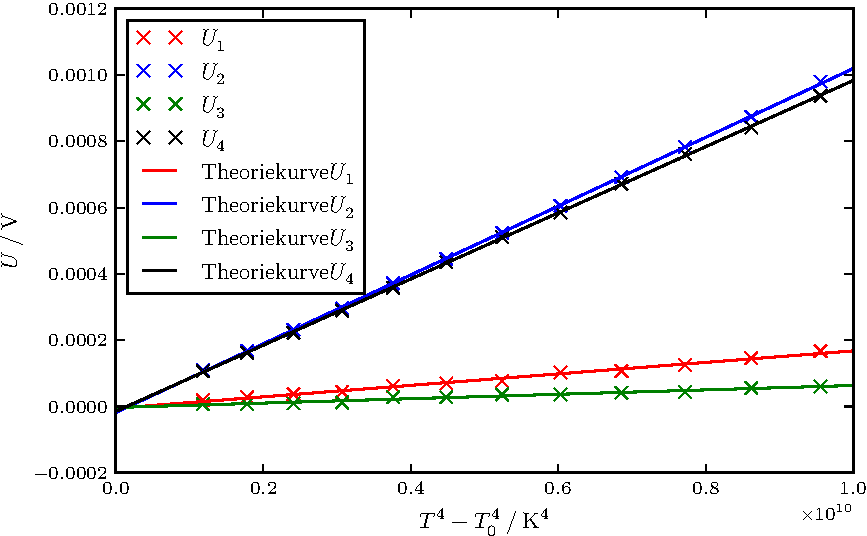
\includegraphics{plot.pdf}
%  \caption{Plot.}
%  \label{fig:plot}
%\end{figure}
%
%\begin{table}
%  \centering
%  \caption{Beispieltabelle}
%  \label{tab:tabelle_beispiel}
%  \sisetup{table-format=1.2}
%  \begin{tabular}{c c}
%    \toprule
%    {$a [\si{\second}]$} & {$b [\si{\kelvin}]$}\\
%    \midrule
%    1.0000  & 11.00 \\
2.0000  & 12.00 \\
3.0000  & 13.00 \\
4.0000  & 14.00 \\
5.0000  & 15.00 \\
6.0000  & 16.00 \\
7.0000  & 17.00 \\
8.0000  & 18.00 \\
9.0000  & 19.00 \\
10.0000 & 20.00 \\

%    \bottomrule
%  \end{tabular}
%\end{table}
%
%Es ergibt sich
%\begin{align}
%  a &= (0 \pm 0) ~ \si{\joule\per\kelvin\per\gram}
 \\
%\end{align}
%
